\documentclass[10pt,a4paper]{article}

\usepackage[utf8]{inputenc}
\usepackage[T1]{fontenc}
\usepackage[ngerman]{babel}
\usepackage[a4paper,left=10mm,right=11mm,top=10mm,bottom=10mm]{geometry}
\usepackage{xcolor}
\usepackage{graphicx}
\usepackage{tabularx}
\usepackage{array}
\usepackage{enumitem}
\usepackage{hyperref}

\IfFileExists{fontawesome5.sty}{
  \usepackage{fontawesome5}
  \newcommand{\IconMail}{\faIcon{envelope}}
  \newcommand{\IconPhone}{\faIcon{phone}}
  \newcommand{\IconLocation}{\faIcon{map-marker-alt}}
  \newcommand{\IconProfile}{\faIcon{linkedin}}
}{
  \newcommand{\IconMail}{@}
  \newcommand{\IconPhone}{T}
  \newcommand{\IconLocation}{\textbullet}
  \newcommand{\IconProfile}{in}
}

% ------------------------------------------------------------
% HENSOLDT-Farben nach dem Karriereportal (jobs.hensoldt.net).
% Zum Anpassen des CV nur diese Werte ändern.
% ------------------------------------------------------------
\definecolor{CVPrimary}{HTML}{13A256}
\definecolor{CVAccent}{HTML}{13A256}
\definecolor{CVText}{HTML}{222222}
\definecolor{CVMuted}{HTML}{505652}
\definecolor{CVSoft}{HTML}{F6F7F6}
\definecolor{CVRule}{HTML}{D7EAD6}

\hypersetup{
  colorlinks=true,
  urlcolor=CVPrimary,
  linkcolor=CVPrimary
}

\renewcommand{\familydefault}{\sfdefault}
\pagestyle{empty}
\setlength{\parindent}{0pt}
\setlength{\parskip}{0pt}
\setlist[itemize]{leftmargin=4mm,topsep=0.6mm,itemsep=0.25mm,parsep=0mm}

\newcommand{\sidebarsection}[1]{%
  \vspace{3mm}%
  {\normalsize\bfseries\textcolor{CVPrimary}{\MakeUppercase{#1}}}\par
  \vspace{0.8mm}{\color{CVAccent}\rule{\linewidth}{0.6pt}}\vspace{1.1mm}
}

\newcommand{\mainsection}[1]{%
  \vspace{3mm}%
  {\large\bfseries\textcolor{CVPrimary}{\MakeUppercase{#1}}}\par
  \vspace{0.8mm}{\color{CVRule}\rule{\linewidth}{0.6pt}}\vspace{1.2mm}
}

\newcommand{\sideitem}[2]{%
  {\bfseries #1}\par
  {\small #2}\par\vspace{1.2mm}
}

\newcommand{\contactitem}[2]{%
  \makebox[5mm][c]{\textcolor{CVPrimary}{#1}}%
  \hspace{1mm}%
  \begin{minipage}[t]{\dimexpr\linewidth-6mm\relax}
    {\small #2}
  \end{minipage}\par\vspace{1.2mm}
}

\newcommand{\entry}[4]{%
  \begin{tabularx}{\linewidth}{@{}>{\raggedright\arraybackslash}p{0.18\linewidth}@{\hspace{2.5mm}}X@{}}
    {\small\textcolor{CVMuted}{#1}} &
    {\bfseries #2}\hfill{\small\textcolor{CVMuted}{#3}}\par
    #4
  \end{tabularx}\vspace{1.8mm}
}

\newcommand{\compactentry}[3]{%
  {\bfseries #1}\hfill{\small\textcolor{CVMuted}{#2}}\par
  #3\par\vspace{1.7mm}
}

\newcommand{\tag}[1]{%
  \begingroup
  \setlength{\fboxsep}{1.4pt}%
  \colorbox{CVSoft}{\scriptsize\textcolor{CVPrimary}{#1}}%
  \endgroup\hspace{0.7mm}%
}

\begin{document}
\color{CVText}

\begin{minipage}[t]{0.285\textwidth}
  \vspace{0pt}
  \setlength{\fboxsep}{3mm}%
  \colorbox{CVSoft}{%
    \begin{minipage}[t][\dimexpr\textheight-2\fboxsep-5mm\relax]{\dimexpr\linewidth-2\fboxsep\relax}
      \vspace{1mm}
      \centering
      \fcolorbox{CVRule}{white}{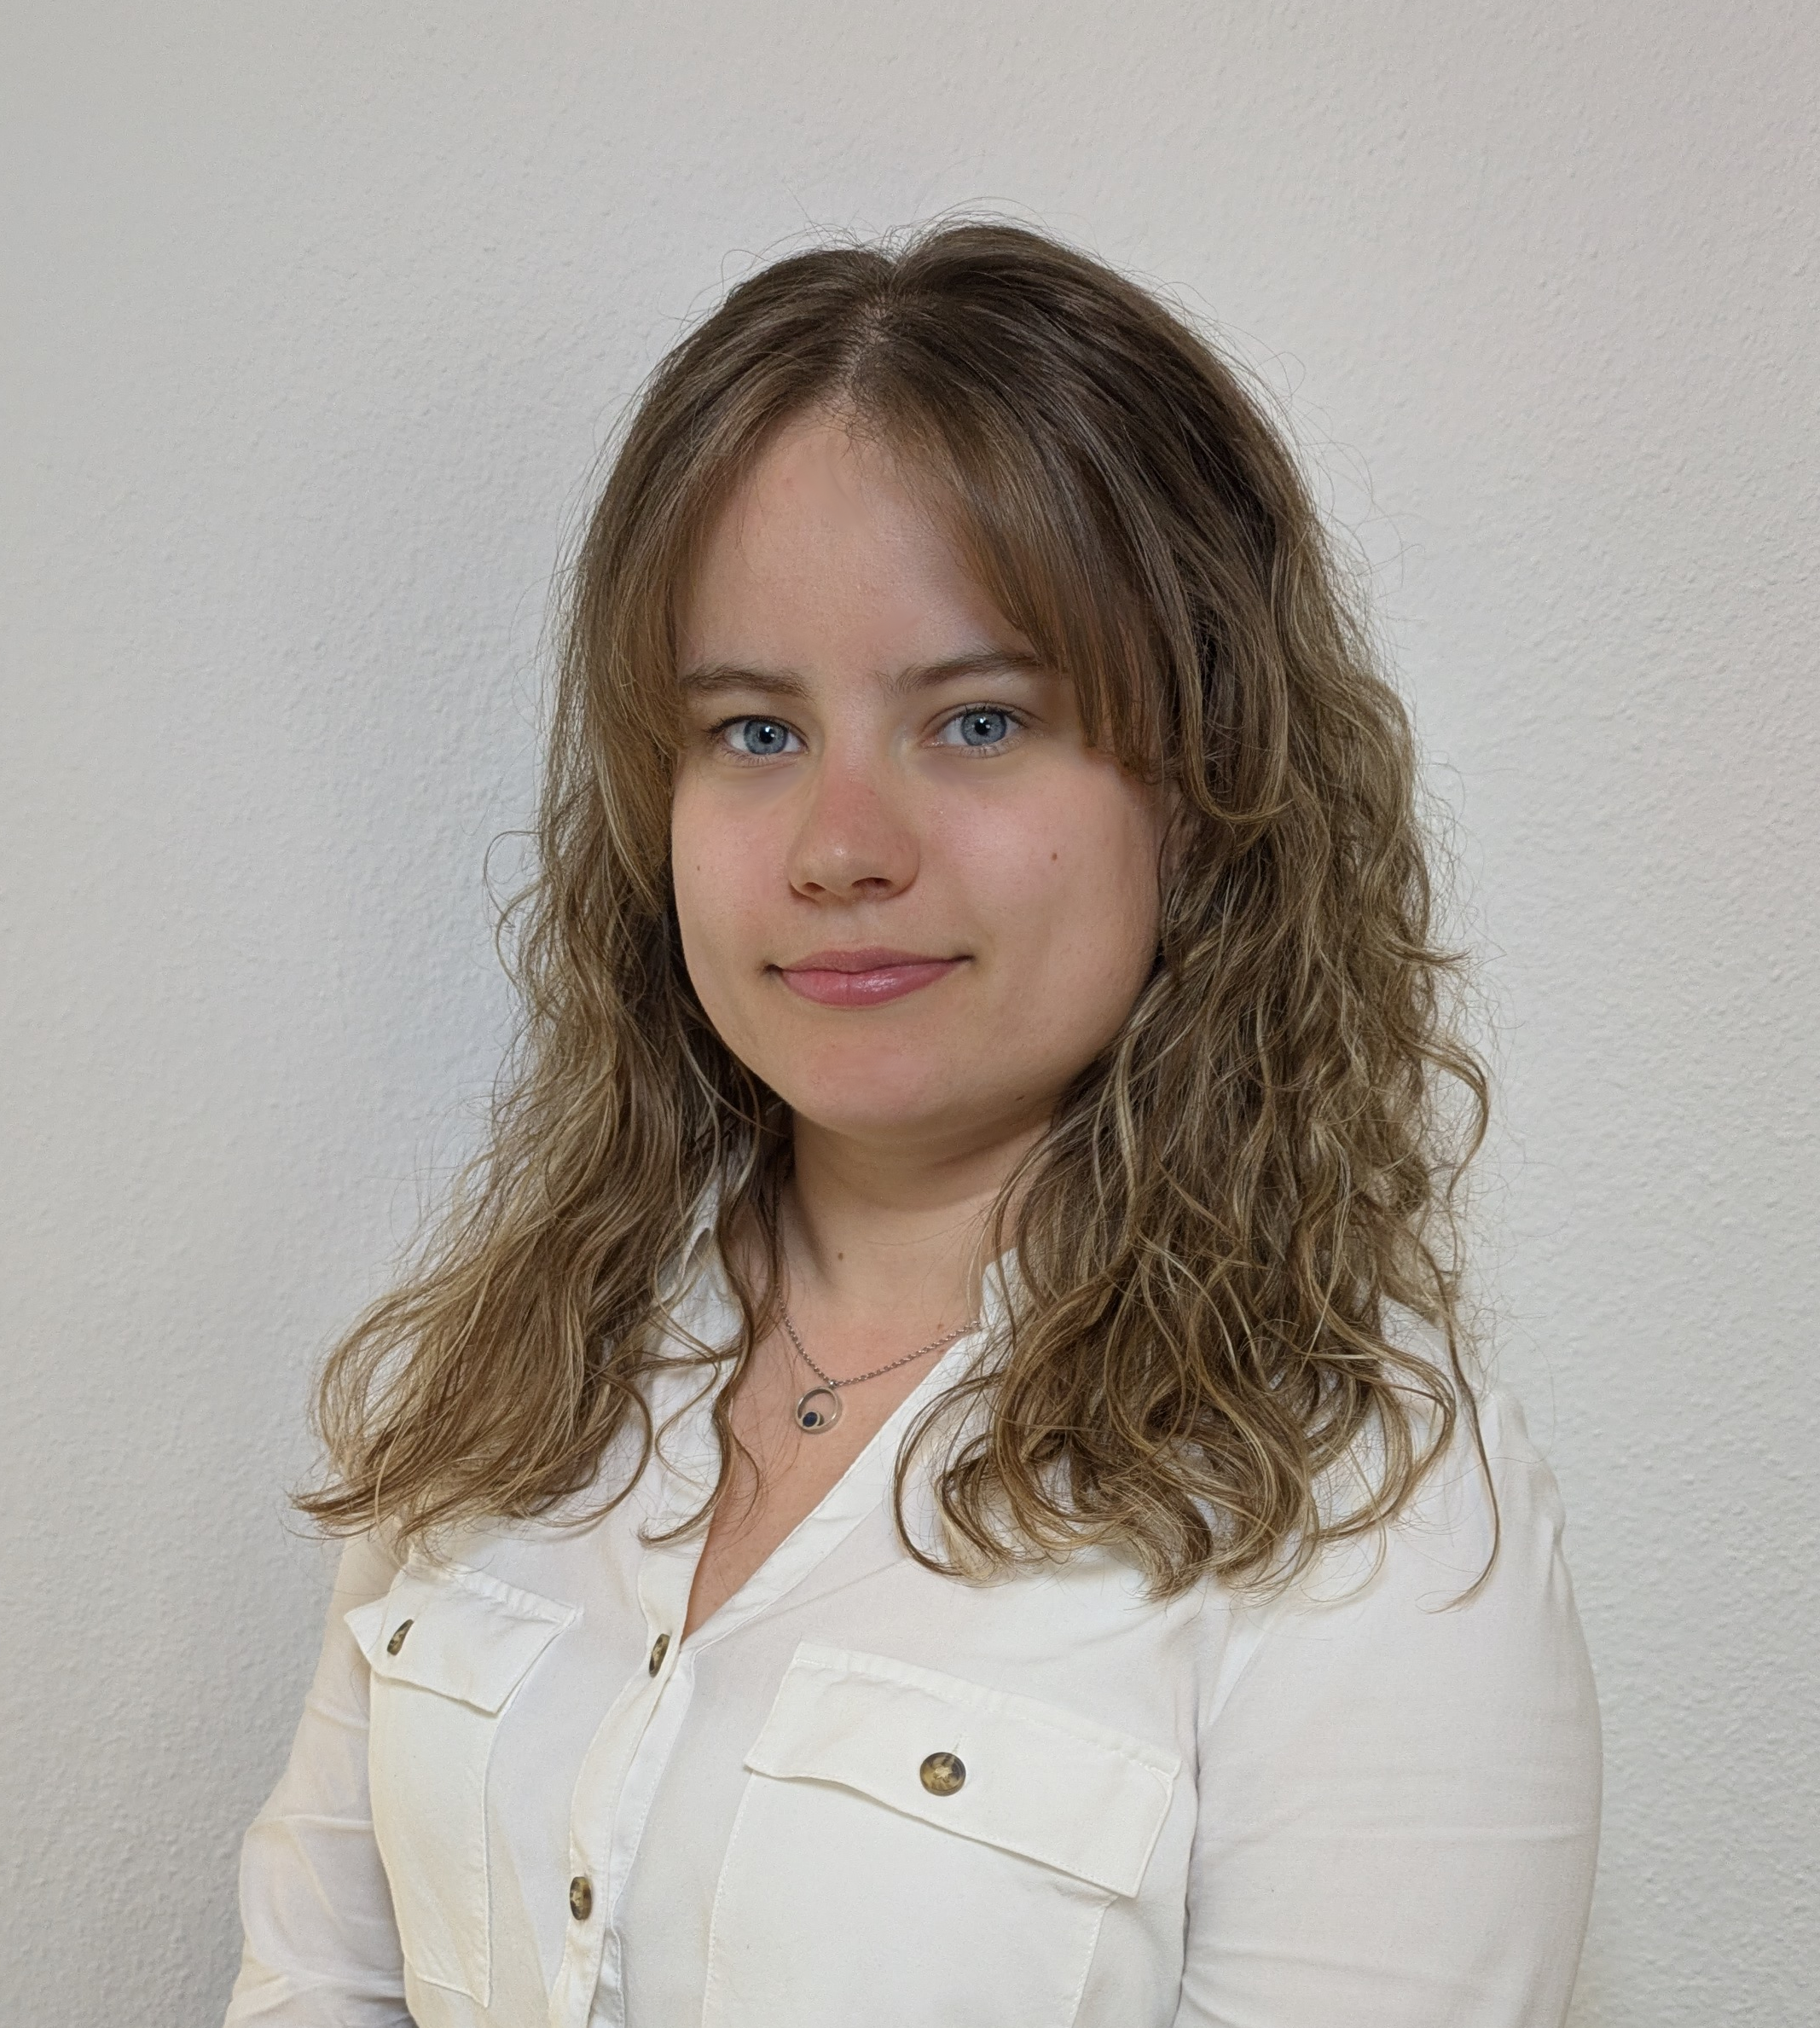
\includegraphics[width=3.55cm,height=4.35cm,keepaspectratio]{Bewerbungsbild.png}}\par
      \vspace{3mm}

      \raggedright
      \sidebarsection{Kontakt}
      \contactitem{\IconMail}{\href{mailto:kontakt@natalieboehm.de}{kontakt@natalieboehm.de}}
      \contactitem{\IconPhone}{+49 1522 1746238}
      \contactitem{\IconLocation}{Aalen}
      \contactitem{\IconProfile}{@natalieboehm2001}

      \sidebarsection{Fähigkeiten}
      \small
      \textbf{Machine Learning}\par
      PyTorch, TensorFlow, NLP, Detektion, Transformer, TensorBoard\par\vspace{1.1mm}
      \textbf{Computer Vision}\par
      CNN, Fine-Tuning, Segmentierung, Klassifikation\par\vspace{1.1mm}
      \textbf{Software}\par
      Python, Webentwicklung, Java, C\#, SQL, Testing\par\vspace{1.1mm}
      \textbf{DevOps}\par
      Docker, CI/CD

      \sidebarsection{Sprachen}
      Deutsch: C2\par
      Englisch: C1\par
      Französisch: B2\par
      Spanisch: B2\par
      Koreanisch: A2, Auslandssemester

      \sidebarsection{Zertifikate}
      AI Leadership\par
      {\small NextEducation}

      \sidebarsection{Freizeit}
      Tanzen\par
      Kampfsport\par
      Private Infrastruktur\par
    \end{minipage}
  }
\end{minipage}
\hfill
\begin{minipage}[t]{0.68\textwidth}
  \vspace{0pt}
  {\fontsize{25}{28}\selectfont\bfseries Natalie Böhm}\par
  \vspace{1mm}
  {\Large\textcolor{CVPrimary}{Computer Vision Engineer}}\par
  \vspace{2.5mm}
  {\small
    An der Schnittstelle von Computer Vision und Softwareentwicklung
    entwickle ich datengetriebene Lösungen für reale Bild- und Prozessdaten: von
    Modelltraining, Evaluation und Fehleranalyse bis zur technischen Integration und
    Automatisierung. Ich bringe fundierte Praxiserfahrung aus dualem Studium und
    Werkstudententätigkeiten mit. IT ist für mich mehr als ein Karriereweg – ein Umfeld, in dem ich
    mich auch privat engagiere und eigene Ideen umsetze.
  }\par

  \mainsection{Ausbildung}

  \entry{10/2024--09/2026}{M.Sc. Machine Learning \& Data Analytics}{HS Aalen}{
    Schwerpunkt: NLP, Deep Learning und Computer Vision\par
    Masterarbeit: AI-based Signal Separation of Friedel Pairs in Crystallography
  }

  \entry{10/2021--09/2024}{B.Sc. Wirtschaftsinformatik}{DHBW / Bosch Stuttgart}{
    Dualer Studiengang mit Fokus auf Application Management\par
    Bachelorarbeit: Anwendung und Evaluation von Domain Adversarial Training in der Ultraschall-Höhenklassifikation
  }

  \entry{09/2012--06/2021}{Abitur}{Nellenburg-Gymnasium Stockach}{}

  \mainsection{Berufserfahrung}

  \entry{04/2025--08/2026}{Werkstudentin}{ZEISS SMT GmbH, Oberkochen}{
    Entwicklung eines Reinforcement-Learning-Agenten für ein Scheduling-Problem;
    Monitoring und Analyse der Maschinenauslastung; KI-gestützte Entwicklung für
    Prototyping, Dokumentation und Review-Workflows.\par
    \tag{Python}\tag{Reinforcement Learning}\tag{AI-assisted Development}\tag{Elastic}
  }

  \entry{10/2024--03/2025}{Werkstudentin}{Robert Bosch GmbH, Stuttgart-Feuerbach}{
    Verbesserung des Asset-Managements mit RFID-Technologien; Evaluation eines KI-Chatbots
    mit internen Tools zur Verbesserung des Knowledge-Managements.\par
    \tag{GenAI-Bots}\tag{Knowledge Management}\tag{Prozessanalyse}\tag{Scrum}
  }

  \entry{10/2021--09/2024}{Duale Studentin}{Robert Bosch GmbH, Stuttgart-Feuerbach}{
    Rotation durch die Abteilungen SIEM, Hadoop, Infrastruktur und Driving Experience mit Fokus auf Parkassistenten, einschließlich eines Praxissemesters in Polen.\par
    \tag{Hadoop}\tag{Infrastruktur}\tag{Splunk}\tag{Python}\tag{Linux}
  }

  \mainsection{Ehrenamtliches \& zusätzliche Projekte}

  \compactentry{Selfnet e.\,V. -- Infrastruktur und Entwicklung}{seit Studium}{
    2. Beisitzerin, Hardwarewartung, DNS-Administration und Mitgliedersupport bei
    Netzwerkproblemen, Entwicklung des Verwaltungssystems sowie Kubernetes-Grundkenntnisse\par
    \tag{Django}\tag{Python}\tag{Podman}\tag{DNS}
  }

  \compactentry{Private Infrastruktur}{privat}{
    Einsatz von Ansible für wiederholbare Konfiguration und Administration eigener Systeme wie z.\,B. Nextcloud oder Home Assistant; Einsatz von Sprachmodellen und eigenes Training von Modellen zur Wake-Word-Erkennung\par
    \tag{Ansible}
  }

  \compactentry{InnoConsult e.\,V.}{ehrenamtlich}{
    Eventmanagement, Design-Thinking-Workshops und Entwicklung von Marketingstrategien für Startups.
  }
\end{minipage}

\end{document}
